\section{Theorie}
\label{sec:Theorie}

% In knapper Form sind die physikalischen Grundlagen des Versuches, des Messverfahrens, sowie sämtliche für die Auswertung erforderlichen Gleichungen darzustellen. (Keine Herleitung)

% (eventuell die Aufgaben)

% Der Versuchsaufbau: Beschreibung des Versuchs und der Funktionsweise (mit Skizze/Bild/Foto)
 
Für diesen Versuch wird Licht als elektromagnetische Welle angenommen, mit der Form 
\begin{equation}
    \vec{E}(x,t) = \vec{E_0} \cdot \cos{\left(k \cdot x - \omega \cdot t - \delta\right)}.
    \label{eq:licht}
\end{equation}
Hierbei ist $k$ die Wellenzahl, $\omega$ die Kreisfrequenz und $\delta$ der Phasenwinkel.
Die Intensität $I$ einer solchen Welle lässt sich über 
\begin{equation}
    I = c \cdot |\vec{E_0}|^2
\end{equation}
berechnen, mit der Konstante $c$.
Werden zwei Wellen dieser Art überlagert, ergibt sich die folgende Gesamtinsentität
\begin{equation}
    I_\text{ges} = 2\cdot c \cdot \vec{E_0}^2 \left(1 + \cos{(\delta_2 - \delta_1)}\right)
\end{equation}
Es ist zu beobachten, dass sich die Wellenintensitäten nicht einfach addieren, sondern ein sogenannter Interferenzterm $2\cdot c \cdot \vec{E_0}^2\cos{(\delta_2 - \delta_1)}$ addiert werden muss.
Durch die Eigenschaften des Cosinus ergibt sich, dass die Gesamtintensität verschwindet, wenn $\delta_2 - \delta_1$ ein ungerades Vielfaches von $\pi$ ist.

Um diese Interferenzeffekt beobachten können, muss kohärentes Licht verwendet werden.
Also Licht dessen Wellen sich alle nach \autoref{eq:licht} verhalten. 
Ein LASER erfüllt diese Bedingung, $k$, $\omega$ und $\delta$ sind bei jeder Welle gleich. 
Überlicherweise wird für die Beobachtung der Interferenzeffekte ein einzelner LASER verwendet, dieser wird wie in \autoref{fig:bild1} in zwei Strahlen aufgeteilt und teilweise umgelenkt.
Wenn die beiden Strahlen wieder gebündelt werden, haben sie eine Phasenverschiebung untereinander.

\begin{figure}
    \centering
    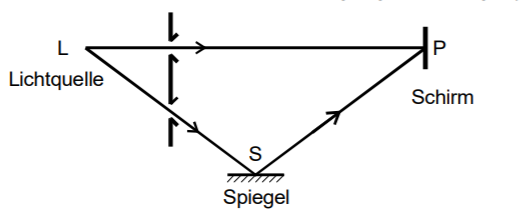
\includegraphics[width=0.4\textwidth]{images/bild1.png}
    \caption{Prinzip der Phasenverschiebung.\cite{V401}}
    \label{fig:bild1}
\end{figure}


Dabei darf der Wegunterschied beider Strahlen nicht zu groß sein, da sonst keine Interferenzeffekte mehr auftreten. Die maximale Länge, bei der noch Effekte auftreten, wird Kohärenzlänge $l$ genannt und kann aus der Wellenlänge$\lambda$ und der maximalen Anzahl Maxima $N$ bei der Phasenverschiebung $\delta$ über 
\begin{equation}
    l = N \cdot \lambda
\end{equation}
berechnet werden.
Allerdings darf der Wegunterschied auch kein ungerades Vielfaches von $\frac{\lambda}{2}$ sein, da die Intensität dann ebenfalls verschwindet.
Gleichzeitig gibt es die Kohärenzzeit $\tau$, diese gibt die Dauer des Emissionsaktes an und kann über 
\begin{equation}
    \tau = \frac{l}{c}
\end{equation}
bestimmt werden. $c$ ist dabei die Lichtgeschwindigkeit der Welle.

Das Michelson-Interferometer basiert auf der Nutzung dieser Interferenzeffekte.
Der allgemeine Aufbau eines solchen Interferometers ist in \autoref{fig:bild2} dargestellt.

\begin{figure}
    \centering
    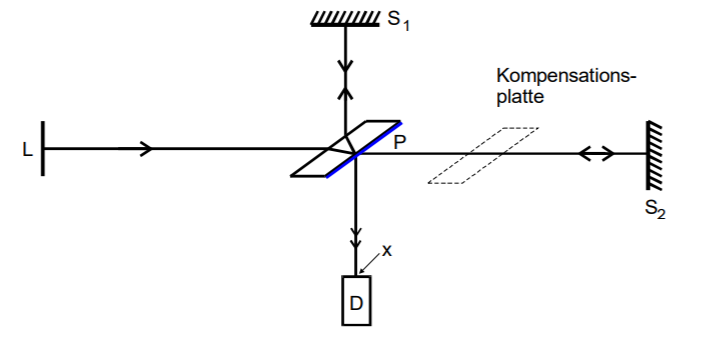
\includegraphics[width=0.4\textwidth]{images/bild2.png}
    \caption{Prinzipieller Aufbau eines Michelson-Interferometers.\cite{V401}}
    \label{fig:bild2}
\end{figure}

Die Lichtquelle $L$ sendet einen LASER aus, der einen semipermeablen Spiegel $P$ passiert, dabei wird ein Teil gebrochen und der andere durchquert ihn unverändert.
Beide Strahlen treffen auf einen Spiegel $S_\text{1}$ oder $S_\text{2}$.
Dort werden sie erneut reflektiert und kehren zum Spiegel $P$ zurück, dort werden sie theoretisch erneut gebrochen, jedoch wird nur der Teil betrachtet, der zum Detektor $D$ läuft.
Sind beide Strahlenwege gleich lang, so besitzen die Strahlen eine Verschiebung von $\frac{\lambda}{2}$, wodurch die Intensität verschwindet.
Um die Gleichheit der Wege zu gewährleisten wird auf der Strahlstrecke zu Spiegel $S_\text{2}$ eine Kompensationsplatte befestigt.
Dies wird getan, da der andere Strahl auf dem Weg zum Detektor $D$ drei mal den Spiegel $P$ passiert, und der andere Strahl nur ein mal. 
Auf diese Weise können die Strahlen angelichen werden.
Der Spiegel $S_\text{2}$ kann nun um die Länge $\Delta d$ verschoben werden, wodurch sich die Weglänge um $w = 2\Delta d$ ändert.
Gleichzeitig ergibt sich folgender Zusammenhang
\begin{equation}
    \Delta d = \frac{z \cdot \lambda}{2}
\end{equation}
$z$ steht für die Anzahl der auftretenden Helligkeismaxima.

Es gibt noch eine weitere Möglichkeit den Wegunterschied zu ändern, so kann ebenfalls auf einem der Strahlenwege ein Medium mit einem anderen Brechungsgrad $n + \Delta n$ eingesetzt werden.
Diese Strecke hat die Länge $b$. 
Der veränderte Aufbau ist schematisch in \autoref{fig:bild3} dargestellt.

\begin{figure}
    \centering
    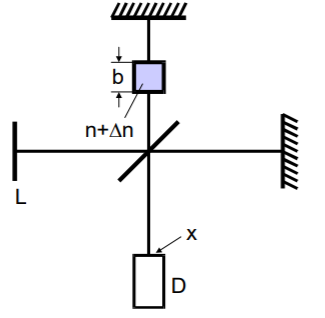
\includegraphics[width=0.4\textwidth]{images/bild3.png}
    \caption{Messung mit Michelson-Interferometers durch Brechungsgradunterschiede.\cite{V401}}
    \label{fig:bild3}
\end{figure}

Es lässt sich der Zusammenhang 
\begin{equation}
    b \cdot \Delta n = \frac{z \cdot \lambda}{2}
\end{equation}
feststellen.
Nun kann der Druck $p$ innerhalb dieses Bereiches mit der Länge $b$ auf $\acute{p}$ gesenkt werden.
Dann gilt ebenfalls
\begin{equation}
    n = \sqrt{1 + f(\lambda)N},
\end{equation}
wobei $N$ die Anzahl der von der Lichtwelle zu Schwingungen pro Volumeneinheit angeregten Moleküle beschreibt.
Für Gase im sichtaren Bereich des Lichts gilt außerdem die Näherung
\begin{equation}
    n = 1 + \frac{f}{2} \cdot N.
\end{equation}
Der Wert für $N$ kann über
\begin{equation}
    N = \frac{p T_0 N_\text{L}}{T p_0}
\end{equation}
berechnet werden.
$p_0$ und $T_0$ sind jeweils Druck und Temperatur bei Normalbedingungen und $N_\text{L}$ ist die sogenannte  Loschmidtsche Zahl.
Der Unterschied es Brechungsindexes $\Delta n$ kann über den Ausdruck
\begin{equation}
    \Delta n = \frac{f}{2} N_\text{L} \frac{T_0}{p_0} \frac{1}{T} (p - \acute{p})
\end{equation}
bestimmt werden.
Nachdem alle Größen eingesetzt werden ergibt sich dann die endgültige Formel
\begin{equation}
    n = 1 + \frac{z \lambda}{2  b } \frac{T}{T_0} \frac{p_0}{p - \acute{p}}.
\end{equation}